\documentclass[border=10pt]{standalone}
\usepackage{pgfplots}
\pgfplotsset{compat=1.17}
\begin{document}
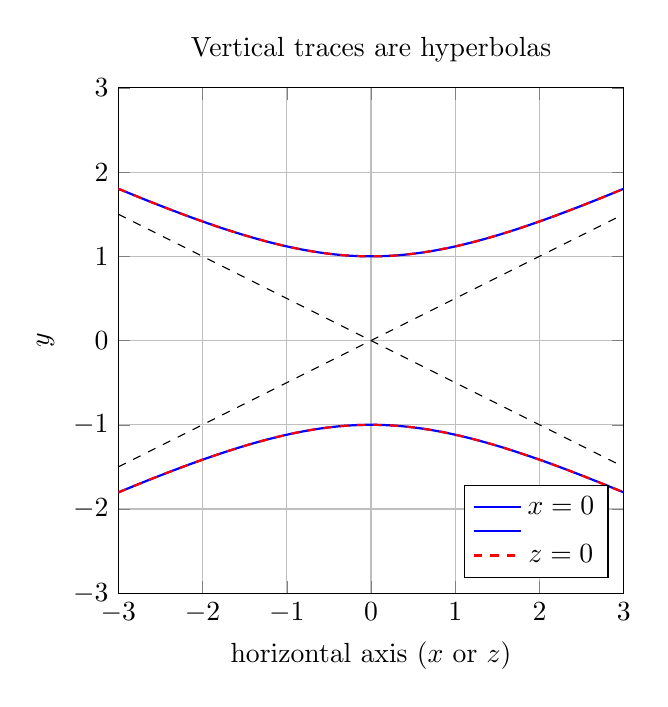
\begin{tikzpicture}
\begin{axis}[
    width=8cm, height=8cm,
    axis equal image,
    xmin=-3, xmax=3, ymin=-3, ymax=3,
    xlabel={horizontal axis ($x$ or $z$)}, ylabel=$y$,
    grid=both,
    title={Vertical traces are hyperbolas},
    legend pos=south east
]
\addplot[blue, thick, domain=-3:3, samples=200]
    {sqrt(1+x^2/4)};
\addplot[blue, thick, domain=-3:3, samples=200]
    {-sqrt(1+x^2/4)};
\addplot[red, thick, domain=-3:3, samples=200, dashed]
    {sqrt(1+x^2/4)};
\addplot[red, thick, domain=-3:3, samples=200, dashed]
    {-sqrt(1+x^2/4)};
\addplot[black, dashed, domain=-3:3, samples=2]{x/2};
\addplot[black, dashed, domain=-3:3, samples=2]{-x/2};
\legend{$x=0$,$ $,$z=0$}
\end{axis}
\end{tikzpicture}
\end{document}
